\documentclass{beamer}

\mode<presentation>
{
  \usetheme{Boadilla}
  % or ...

  \setbeamercovered{transparent}
  % or whatever (possibly just delete it)
}


\title[Tupelo] % (optional, use only with long paper titles)
{Towards Automated Disk Forensics}

\subtitle
{Sub} % (optional)

\author[] % (optional, use only with lots of authors)
{Stuart Maclean \\
University of Washington}
% - Use the \inst{?} command only if the authors have different
%   affiliation.

\date[] % (optional)
{Dec 2014}


\usepackage{graphicx}
%\usepackage{pbox}
\usepackage{tikz}


\begin{document}

%\includeonlyframes{current}

\begin{frame}
  \titlepage
\end{frame}


\begin{frame}{Outline}
  \tableofcontents[pausesections]
  % You might wish to add the option [pausesections]
\end{frame}

%%%%%%%%%%%%%%%%%%%%%%%%%%% %%%%%%%%%%%%%%%%%%%%%%%% %%%%%%%%%%%%%%%%%%%%%%%

\section{Managed and Unmanaged Disks}

\begin{frame}{Managed and Unmanaged Disks}

\end{frame}

%%%%%%%%%%%%%%%%%%%%%%%%%%% %%%%%%%%%%%%%%%%%%%%%%%% %%%%%%%%%%%%%%%%%%%%%%%

\begin{frame}{Initial Data Acquisition}

\begin{center}
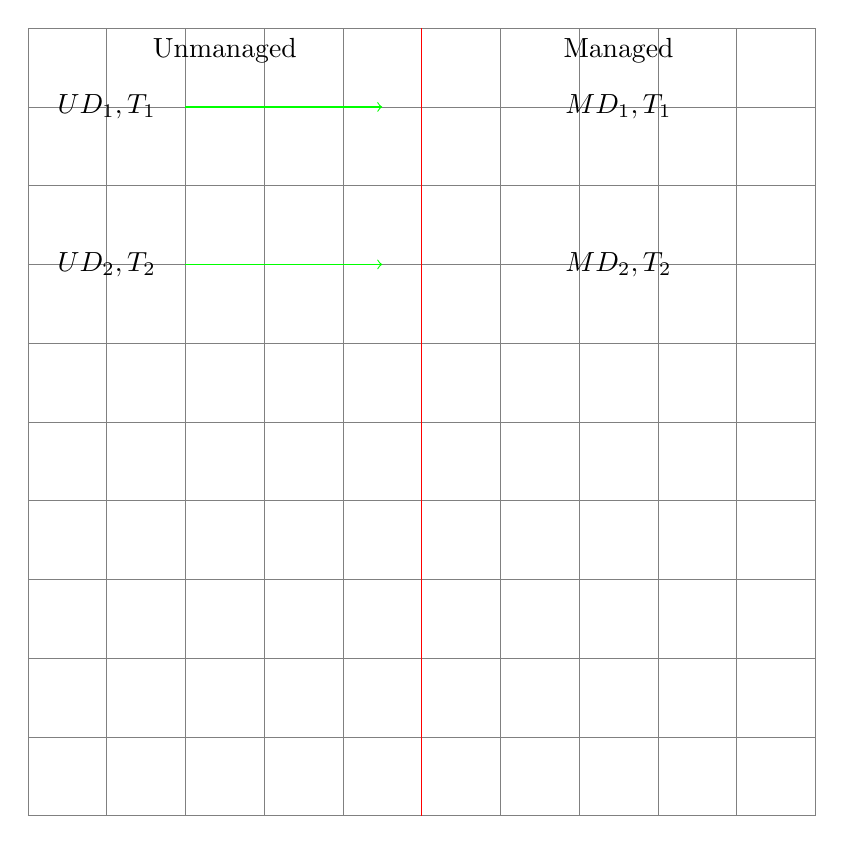
\begin{tikzpicture}

\draw[help lines] (0,0) grid (10,10);

\draw [red] (5,0) -- (5,10);
\node [below] at (2.5,10) {Unmanaged};
\node [below] at (7.5,10) {Managed};

%% First putdata, user 1
\draw [->, green] (2,9) -- (4.5,9);
\node at (1,9) { $UD_{1},T_{1}$ };
\node at (7.5,9) { $MD_{1},T_{1}$ };

%% First putdata, user 2
\draw [->, green] (2,7) -- (4.5,7);
\node at (1,7) { $UD_{2},T_{2}$ };
\node at (7.5,7) { $MD_{2},T_{2}$ };

\end{tikzpicture}
\end{center}

\end{frame}

%%%%%%%%%%%%%%%%%%%%%%%%%%%%%%%%%%%%%%%%%%%%%%%%%%%%%%%%%%%%%%%%%%%%%%%%%%%%

\begin{frame}{Subsequent Data Acquisition}

\begin{center}
\begin{tikzpicture}

%\draw[help lines] (0,0) grid (10,8);

%% Existing putdata
\draw [->] (1,1) -- (4,4);
\node [below] at (1,1) { $UD_{1},T_{1}$ };

%% Second putdata
\draw [->] (3,0.5) -- (4.5,4);
\node [below] at (3,0.5) { $UD_{1},T_{3}$ };

\draw (4,4) rectangle (6,6);

%% Existing putdata
\draw [->] (9,1) -- (6,4);
\node [below] at (9,1) { $UD_{2},T_{2}$ };

%% Second putdata
\draw [->] (7,0.5) -- (5.5,4);
\node [below] at (7,0.5) { $UD_{2},T_{4}$ };

\end{tikzpicture}
\end{center}

\end{frame}

%%%%%%%%%%%%%%%%%%%%%%%%%%%%%%%%%%%%%%%%%%%%%%%%%%%%%%%%%%%%%%%%%%%%%%%%%%%%

\begin{frame}{Stored Attributes Accompany Data}

\begin{center}
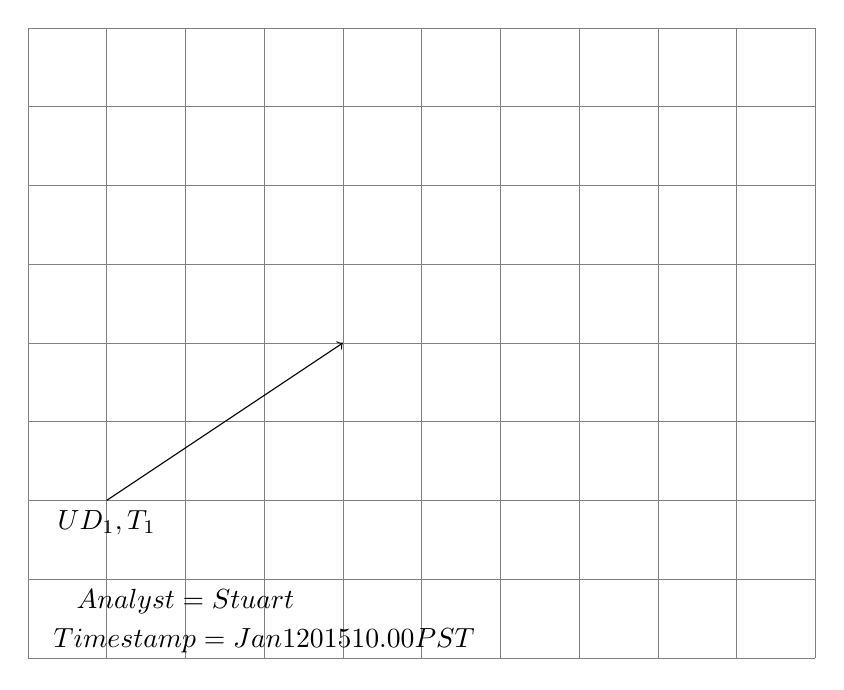
\begin{tikzpicture}

\draw[help lines] (0,0) grid (10,8);

%% Existing putdata
\draw [->] (1,2) -- (4,4);
\node [below] at (1,2) { $UD_{1},T_{1}$ };

%% Attach attributes
\node [below] at (2,1) { $Analyst = Stuart$ };
\node [below] at (3,0.5) { $Timestamp = Jan 1 2015 10.00 PST$ };

\end{tikzpicture}
\end{center}

\end{frame}


\end{document}

% eof
